\chapter[T'aak̲ú Téix̲'i - The Heart of the Taku]{\vspace{-25pt}T'aak̲ú Téix̲'i - The Heart of the Taku:
A multifaceted place name from the Taku River Tlingit First Nation
}

\sethandle{10125/24841}

% \usepackage[
% 	doi=false,
% 	backend=biber,
% 	natbib=true,
% 	style=biblatex-sp-unified,
% 	citestyle=sp-authoryear-comp]{biblatex}
%\usepackage[style=ldc.bst]{biblatex}




% Author last name as it appears in the header
\def\authorlast{Schreyer}

% change author in three references below to the actual author name so that this name is unique and matches the \label commands just below and at the end of the chapter
\renewcommand{\beginchapter}{\pageref{schreyer-ch-begin}}
\renewcommand{\finishchapter}{\pageref{schreyer-ch-end}}
\label{schreyer-ch-begin}



\thispagestyle{firststyle}

\chapauth{Christine Schreyer}
\affiliation{University of British Columbia, Okanagan Campus}

\authortoc{Christine Schreyer}

\section{Introduction}

The traditional territory of the Taku River Tlingit First Nation stretches across northwestern British Columbia into the Yukon and Alaska and encompasses the watershed for which the community is named –the Taku River. This paper examines the multi-faceted use of one place name from the locale of the Taku River, an island known as T'aak̲ú Téix̲'i or the Heart of the Taku. This name serves multiple roles within the community. It is a border marker, but it is also a central point or the “heart” of the community’s territory. The name and a series of metaphors associated with it are also used to invoke principles of stewardship and protection of the land, or what I have referred to as “performatives of stewardship” (Schreyer 2016). The specific locale, T'aak̲ú Téix̲'i, can also be examined using Thornton’s (2011) model for understanding ecotopes, which he describes as the “smallest ecologically-distinct landscape features” (Hunn and Meilleur 2010: 15ff), which hold cultural significance (Thornton 2011: 276).

The island T'aak̲ú Téix̲'i is found on the Alaskan side of the international border between British Columbia and Alaska, but as Louise Gordon states, “the Elders and our ancestors always believed that the rivers, the watersheds, are the borderlines. They didn’t say borderlines, but for them it was the rivers [that were important]” (Gordon L., interview 2006). Kari’s extensive research on Athabaskan place names, as described these mapping systems based on drainage systems as “hydronymic districts” (Kari 1996a). For example, in their research on Tlingit and Haida Land Rights and Use, Goldschmidt and Haas documented that:

\begin{quote}
The original home of the Taku people was on the Taku River. After the establishment of the international boundary, the Taku Tlingits split into two groups, one living upstream on the shores of Lake Atlin, and the other remaining on the coast. The two groups still recognized their unity and maintained contact (Goldschmidt et al 1998: 41).
\end{quote}

As well, despite this imposition of the boundary, the members of the Taku River Tlingit First Nation still use the river on both sides of the border and know the land there intimately. \ Thornton writes, “Many Tlingit place-names are evocative of the mythical and historic past, in so far as they serve to cement the traditional relationship between a particular group or clan and the territory that continues to sustain them” (2008: 102). As will be explained below, the place name T'aak̲ú Téix̲'i or the Heart of the Taku comes from a mythohistoric story about how the landscape of the Taku River was formed, and, therefore, it is one place that illustrates the long-lasting and sustaining connection community members have with the Taku River. Recently, however, the use of the toponym has also been extended to include another locale, a BC Parks Conservancy called the Taku River/T’akú Téix’ Conservancy.\footnote{Consistency in spelling remains a challenge for this community where very few Elders are fluent in Tlingit and none of the Elders have ever been schooled in Tlingit literacy. For this reasons, and others that will be noted below, spelling of the name T'aak̲ú Téix̲'i is inconsistent. } In many colonial nations, place names that are layered on top of one another create a stratigraphy of history (Schreyer 2014) where settler names sit on top of indigenous names. While this is also true in Taku River Tlingit territory (Schreyer et al. 2014), in this specific example, the community has chosen to extend a well-known and important place name laterally, to a different terrain and for a new purpose, and in this manner the place name T'aak̲ú Téix̲'i has become even more tied to stewardship since it is used for a conservancy to protect the land.

Prior to this use of the Tlingit name, T'aak̲ú Téix̲'i, as a form of stewardship, imbricated English metaphors tied to the Heart of the Taku have also been used by community members to assert their stewardship over their lands and in their traditional territory. Following ideas from Mac Cormac on the role of metaphors as performatives, as well as Thornton (2012, 2011, 2008) on metaphor and anatomical connection in Tlingit place-naming practices and the concept of ecotopes, I trace the use of the Heart of the Taku from Mrs. Nyman’s telling of the place name’s origin (Nyman and Leer 1993) to how the name and the ideas associated with the name are used in contemporary times (2014).

\section{Background on the Taku River Tlingit First Nation}

Originally designated by the government of Canada as the Atlin Band, after the large lake (Áa Tlein in Tlingit) on the shores of which their government offices are now located, the Tlingits of northwestern British Columbia began to self-identify to outsiders as people of the Taku River in the early 1980s in association with the start of land claims negotiations in the community. As Alice Carlick told me in an interview from my doctoral research, “a lot of us didn’t like [the name Atlin Band] because we are matrilineal and we do come from the Taku River” (Carlick, A., interview 2006). The Taku River has long been a locality of great importance for the Taku River Tlingit in terms of culture, including economics, politics, social cohesion, and healing. Therefore, the community continues to assert their stewardship over their lands, and this river, in many ways. For instance, in 1999, the Taku River Tlingit First Nation began working with the Round River Organization, a conservation group, in order to develop a sustainable land plan, also known as the Conservation Area Design, to further strengthen their argument for stewardship over their lands and to support their court-case against the mining company, Redfern Resources, that wanted to build a road through the heart of their traditional territory. This case was heard at the Supreme Court of Canada in 2004 and, although the Taku River Tlingit First Nation lost the case on an appeal, their case set legal precedence on issues of consultation. In 2003, the community published the beginnings of a land plan (the Conservation Area Design and a Vision and Management Document).

Since 2003, the Lands and Resources department has released other documents that illustrate their stewardship of their lands. These include the Taku River Tlingit First Nation Mining Policy (2007); the map of the Taku River Tlingit Tlatsini or ‘The Lands That Keep Us Strong’ (2009); and Wóoshtin wudidaa - Atlin Taku Land Use Plan (2011). The Wóoshtin wudidaa - Atlin Taku Land Use Plan is a unique and historic example of government-to-government negotiations that was signed by the province of British Columbia and the Taku River Tlingit First Nation, which according to one news source “balances stewardship with development” (ICTMN 2011). Both the Vision and Management Documents (2003) and the Wóoshtin wudidaa - Atlin Taku Land Use Plan include statements that support the use of Tlingit language, and Tlingit place names in particular. This is important to note since Tlingit is not the everyday language of the community members and very few fluent speakers of the language remain in the community (TRTFN-ALI 2014).

Therefore, while some people do know the Tlingit name of T'aak̲ú Téix̲'i (Heart of the Taku), this name is also used in a variety of different ways in English as well, as I describe below. In addition, since there is a desire in the community for language revitalization, the community members have developed various programs and projects to help encourage more Tlingit language use. Among these is the development of an interactive, participatory map, which records Tlingit place names, the English meaning of the Tlingit place names, audio recordings of Elders saying the place name, and finally, photos of the place. This website was developed through a joint research project between the Taku River Tlingit First Nation and researchers at the University of British Columbia, including myself, in order to: 1) support Tlingit language revitalization and 2) illustrate the community’s continued stewardship over their lands. I describe this website in more detail below, but first turn to the origins of the name T'aak̲ú Téix̲'i and the Heart of the Taku.

\section{Remembering the Giants’ Battle}

One of the first published records of the Heart of the Taku comes from Mrs. Elizabeth Nyman, a respected Taku River Tlingit Elder who passed away in 1999. Mrs. Nyman co-authored the book \textit{Gágiwduł.àt: Brought Forth to Reconfirm - The Legacy of a Taku River Tlingit Clan}\footnote{ For the publication of this book, Jeff Leer developed an alternate Tlingit writing system that was used in Atlin until recently, which continues to be used in some areas of the Yukon. In 2006, the Taku River Tlingit Elders Council voted to start using the orthography popularized by Sealaska Heritage Institute. Therefore, in this article all Tlingit writing is in this orthography, often known as the Coastal Orthography. Quotes from Mrs. Nyman’s book, however, retain their original spelling.}  with linguist Jeff Leer (Nyman and Leer 1993). In this book, the transcription of the story entitled “The Battle of the Giants” appears in the both Tlingit and English. This story, which Mrs. Nyman told in 1988 in Tlingit, describes the mythohistoric battle that two giants (Was’as’ê and Łkùdasêts’k) engage in over the Taku River. Eventually, Was’as’ê rips Łkùdasêts’k apart and throws pieces of his body all over the Taku. He declares, “Let Łkùdasêts’k’s heart become the Heart of the Taku” (Nyman and Leer 1993: 5), and to this day that heart, the island, remains in the Taku River. The story of the T'aak̲ú Téix̲'i also appears in Mrs. Nyman’s telling of “T’aakhu Yan Yédì Dat Shalnik” or the history of the Taku Yanyeidí\footnote{Yanyeidí is the clan name spelled in the Sealaska orthography and will be the spelling used when not referring to a specific item from the Nyman and Leer (1993) book. } clan, which she recorded in 1984. Yanyeidí is the wolf clan of the wolf moiety to which Mrs. Nyman belonged.\footnote{ Yán is the Tlingit word for Western Hemlock (Crippen 2010), which is what the clan’s house was built of on the Taku River. It also appears in the name of the mountain K’iyán (Hemlock grows around the bottom).} Throughout this story, Mrs. Nyman again describes the giant’s battle because it is significant to the history of the Yanyeidí people who built their clan houses on the Taku River. In this story Mrs. Nyman describes in more detail what the pieces of Łkùdasêts’k look like when he is ripped apart and where they landed, including his head (which is also an island), and his windpipe (on a mountain), which has water so cold flowing from it that no one can drink it. About his heart, she says:

\begin{quote}
His heart he yanked out and threw it into the Taku River. There is a small island there, perhaps a little larger than this room, stretched out so; only short grass grows on it. “This will be the Heart of the Taku”, said Was’as’ê....This is what my father-in- law used to tell us, since he was a young boy they told him that it’s still the same as ever. For some reason it never drifts away, the Heart of the Taku? I suppose it is still there to this day. [Nyman and Leer 1993: 29]
\end{quote}

I have been working with the Taku River Tlingit First Nation since February of 2005 on issues relating to language and land, including place names and their importance (Schreyer et al 2014). However, I have never heard this story told; I have only read Mrs. Nyman’s version. This is not to say that community members do not know the story and the significance of T'aak̲ú Téix̲'i\textbf{. }For instance, Elder Jackie Williams, Mrs. Nyman’s oldest son, mentions this island in his story about the forging of the peace treaty and border between the Taku River Tlingit and their Tahltan neighbors to the south. In one section of the story, he describes the Heart of the Taku as a border marker between inland and costal Tlingit people. He says, “\textit{T’aakú Téix’i} marks the limit to which the ocean backs the river water up during high tide, and so is a marker of the boundary between the Taku Tlingit and the \textit{Éil’ ká ku.oowu Lingít }(“salt water people” or coastal Tlingit people)” (Williams 2013). As well, in an interview that I conducted with Louise Gordon, she described the Heart of the Taku as being a place that is of special importance to her and the community as a whole. She said:

\begin{quote}
Down the Taku there’s an island and it’s kind of shaped like a heart and they call it “The Heart of the Taku”, and [the elders] believe that if that island goes away or if someday it will erode then the Taku will not be the same. [Knowledge] like that is probably most important to us. [Gordon interview 2006]
\end{quote}

This knowledge is part of the reason, why the Taku River Tlingit First Nation has worked so hard to protect their land, and specifically, the Taku River.

\section{Locating the Heart}

As described above, T'aak̲ú Téix̲'i and the Heart of the Taku became a central point of focus when the Taku River was jeopardized by a major development in the early 1990s. Redfern Resources, a mining company, wanted to build a road through the community’s territory, which, if constructed, would have caused a huge impact on an otherwise undeveloped large portion of their territory and would have disrupted their traditional way of life. A community made film from this time period states that Redfern Resources wanted to:

\begin{quote}
Re-open a base-metal mine on the east bank of the Tulsequah River, near the Alaska border. The Tulsequah’s glacial waters empty into the Taku...the mine’s reopening [would have cost] more than \$140 million, and \$33 million of which would have gone to construct a 160-kilometre-long, all season road through \textit{the heart} of the TRTFN’s traditional territory.\footnote{Tulsequah is an anglicized spelling and pronunciation of the Tlingit name Taaltsux̲éi, which means root garden. This place was the site of a Tlingit village (see \url{trt.geolive.ca}). } [Taku 1997: 1-2, emphasis added]
\end{quote}

This first battle with mining companies over the river ended in 2004 when the community lost their court case against Redfern on an appeal to the Supreme Court of Canada (SCC 2004 74). More recently, however, the community has filed another lawsuit to protect their river, against Chieftain Metals Inc., which has replaced Redfern Resources as the mining company operating the Tulsequah Chief Mine on the Taku River. The current issue is that the province of British Columbia renewed the certificate of the mine without consulting with the First Nation, as legally required (Rivers Without Borders 2014). On July 24\textsuperscript{th}, 2014, a verdict on this suit was rendered; “The Honourable Justice George Macintosh has ruled that the BC government breached its duty to consult the Taku River Tlingit First Nation when making a critical determination regarding the Tulsequah Chief Mine” (Ecojustice 2014). Since this announcement last summer, the British Columbia Ministry of Environment has determined that the Tulsequah Chief Mine project has been substantially started and the company is therefore permitted to continue the development of the mine (Canadian Press 2014).

However, in both court cases, the community and their supporters make reference to the Taku River as being the “heart” of Taku River Tlingit Territory. For example, the Rivers Without Borders media release on the recent court case states, “The proposed Tulsequah Chief mine is in the \textit{heart} of the Taku River Tlingit’s traditional territory on the banks of the Tulsequah River, a major tributary to the Taku River, and just upstream of the Alaska/BC border” (RWB 2014, emphasis added). While the phrase “the heart of the territory” calls to mind the English synonym for “the center of the territory”, community members often understand this to have a polysemic or double meaning, which includes reference to the English version of the island’s name. The island, the Heart of the Taku, then is iconic of the whole of the river. For example, when I met Terry Jack, a Taku River Tlingit fisherman, for the first time in the summer of 2006 I explained that I was researching the connection between language and land for Taku River Tlingit community members and the first thing he asked me was, “But, you’ve never been down river? You’ve never been to the Heart of the Taku?”\textsuperscript{ }(Schreyer field notes 2006). The double question about down river (an often used phrase to refer to the Taku river) immediately followed by “the Heart of the Taku”, is an excellent example of this extended use of the meaning that has moved from the Tlingit place name T'aak̲ú Téix̲'i to the English translation Heart of the Taku, and then to the extended English meaning of “center”. Not only has the name itself been extended with a new linguistic meaning, but it has also been extended on the land. In particular, the name has also come to be a form of social action and stewardship is in the recent development of a BC Parks Conservancy called the Taku River/T’akú Téix’ Conservancy. Established on June 22\textsuperscript{nd}, 2012, the BC Parks website provides the following information about how this area developed:

\begin{quote}
Taku River/T’akú Téix’ Conservancy was established as a result of the Wóoshtin Wudidaa Atlin Taku Land Use Plan and Taku River Tlingit First Nation Strategic Engagement Agreement. \\

This conservancy encompasses the BC portion of the Taku River main stem from the Alaska border to the confluence of the Nakina and Inklin Rivers. The Taku River Tlingit First Nation has a deep and significant cultural attachment to the Taku River, reflecting a long history of use, occupation and spiritual connection. The Tlingit name (T’akú Téix’) means “Heart of the Taku”. The conservancy is located approximately 65 kilometers south of Atlin.\footnote{ Nakina is an anglicized spelling and pronunciation of the Tlingit place name Naak’ina.áa Héeni (the lower Nakina River from the confluence with the King Salmon River, known as T’á Héeni in Tlingit), which was named for an old village in this area. Inklin is an anglicized spelling and pronunciation of Héen Tlein, meaning “big river” in Tlingit (see: trt.geolive.ca). } (\url{http://www.env.gov.bc.ca/bcparks/explore/cnsrvncy/taku-rv/})
\end{quote}

A significant point from this description is that this conservancy is located within the Canadian side of the Taku River, despite the fact that the original T'aak̲ú Téix̲'i is located on the Alaskan side. T'aak̲ú Téix̲'i and the English, Heart of the Taku, therefore, have numerous and extended meanings within this community.

As Kari has written about the general symbolic Athabaskan geography, “The place names appear in networks and constitute cognitive maps. The place names/signs have had several functions – to facilitate memorizability, and way-finding, to mark travel corridors, to represent land use agreements, or to mark band boundaries” (1996b: 464).\footnote{ I am honored to be included in this volume dedicated to the work of James Kari. His thorough examination of Athabaskan place names has long been an inspiration for my own work. } This can be seen to be true for this Tlingit place name, which is a key locale in a highly significant travel corridor for Taku River Tlingit people. The name is also used to represent contemporary and past land agreements and to mark the boundary between inland and coastal Tlingit peoples. Beyond this an interesting and different set of extended meanings have developed in this community, which are tied to the origins of the Tlingit place name T'aak̲ú Téix̲'i. According to Mrs. Nyman’s story, the island T'aak̲ú Téix̲'i is Łkùdasêts’k’s heart and a set of metaphors related to this anatomical organ are also found in use amongst Taku River Tlingit community members in English.

\section{Of Hearts and Blood}

Within a booklet that was co-written by the Taku River Tlingit First Nation and BC Wild (a conservation group) in support of the Taku River Tlingit First Nation’s first court case, examples of this extended set of metaphors are present. This booklet (see Figure1), printed in 1997, is entitled, “Taku: Will a short-lived mining project sever the \textit{bloodline }of the Tlingit people?” (1997: cover, emphasis added).

\begin{figure}
    \centering
    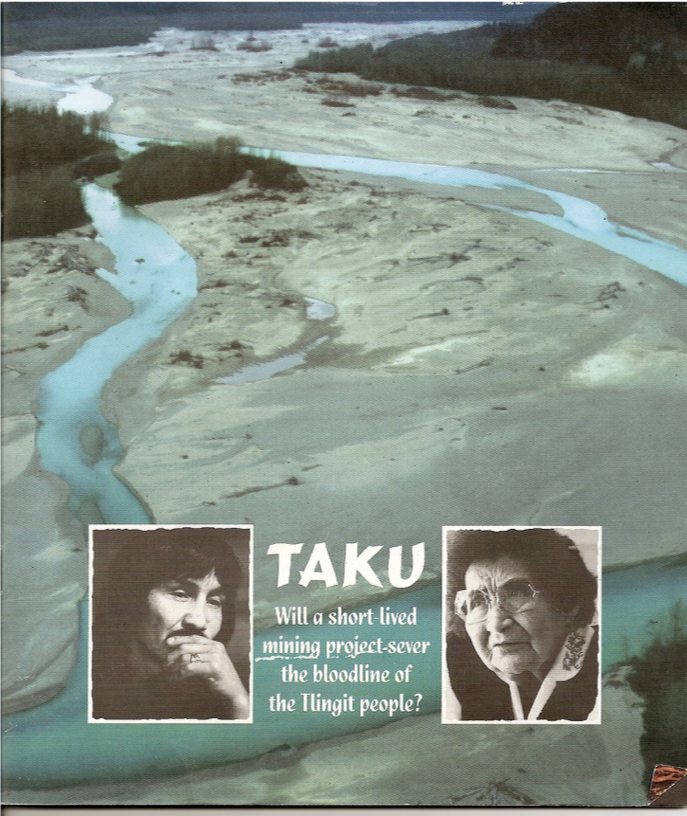
\includegraphics{figures/schreyer-fig1}
    \caption[width=0.5\textwidth]{Taku pamphlet (1997) – the many veins of the Taku River. Bryan Jack, Crow Director (left), and Antonia Jack, Crow Elder (right), are shown as well.}
    \label{schreyer-fig1}
\end{figure}




Similar to the polysemic meanings that the term “heart” holds, the word “bloodline” has multiple meanings in this context for Taku River Tlingit community members as well. English speakers may first think of veins or arteries and the connection to the heart, but veins are also used to describe rivers. The Taku River has many different veins (as seen in Figure 1), but importantly the veins of this river or the bloodlines are those that connect to the Heart of the Taku, to the island. As well, bloodlines in English may also cause English speakers to think of their familial relations. In this case, as Tlingit communities are matrilineal, bloodlines are tied to clans and clans are tied to places. Thornton describes clans as “oldest and most basic unit of Tlingit social structure and the foundation of both individual and group identity” (2008: 46-7), and he goes on to discuss the relationship between clan and place in his book \textit{Being and Place among the Tlingit.} He writes:

\begin{quote}
The linguistic homology between clan and place leads to other metaphoric associations, too. Two images are especially poignant: place/clan as protector and place/clan as provider...in a metaphor of sustenance, the Tsaagweidí can allude to their connection with the key resource, harbor seal (tsaa), found in their place of origin, Hood Bay (Tsaagwáa, “Seal Ice Floes”). Such metaphors are skillfully blended in the context of visual and verbal art. [Thornton 2008: 54]
\end{quote}

The Heart of the Taku is a key place in the history of the T'aak̲ú K̲wáan; the island and the river help to sustain the whole community, but it is of particular importance for community members from the Yanyeidí clan, specifically, whose clan houses were originally built on the Taku (Thornton 2012; Goldschmidt et al 1998).

However, within the text of this booklet, yet another meaning is provided for bloodlines. The Taku River Tlingit First Nation fisheries manager from 1997, Cecil Anderson, describes “the Taku’s salmon as the Tlingit’s \textit{bloodline}” (1997: 8, emphasis added). Fish are hugely important to both the economy of the community and the subsistence of community members. For instance, the salmon from the Taku River is sold by the community-owned and run company, Taku Wild, which sells smoked salmon from the Taku River around the world. The profits from this company support conservation efforts and land planning. On their website it is written, “Our home is this land. Our spirits, lives, and hearts have been shaped here, and we will care for our land just as our ancestors have instructed us” (Taku Wild 2014).

As well, the Taku River Tlingit First Nation currently practice what is known as “food fishing” or the community fishing by Taku River Tlingit members for the rest of the community living in Atlin and Whitehorse. A variety of salmon species are found in the Taku River, including Sockeye, Coho, and Chinook each year (TRTFN 1997), and these are all distributed throughout the community by the fisheries department. I have been in the community when the fish is distributed, and it is always an exciting time! People try to get their favorite type of fish; families join together to share and process the fish, which always arrives whole. The fish is filleted and special parts are laid aside: the head, the fins, and tails (see Figure 2). Due to Atlin’s isolation (it is a 2 hour drive from Whitehorse, Yukon down a windy gravel road), store bought food can often be more expensive than in the city and perishable items often spoil quickly. The salmon then are a healthy source of food, but there is also a spiritual or emotional connection to food that comes from the land. Even in the Taku River Tlingit’s constitution (1993), it is written, “It is the land from which we come that connects all life. Our land is our \textit{lifeblood}” (as quoted in TRTFN 2003, emphasis added). Terry Jack, a Taku fisherman mentioned earlier, is quoted in the Lands and Resources Vision and Management Document - Hà t\_tátgi hà khustìyxh - Our Land is Our Future (2003), his feelings on the salmon that feeds the community:

\begin{quote}
The fish to our people is one of our \textit{lifelines.} And not only that it’s so sacred to our people. It’s a food that represents us as Tlingits...when I think of Taku fish, I think of it as coming from the \textit{heart of the Tlingit country}. [TRTFN 2003: 60, emphasis added]
\end{quote}
\noindent
An interesting chain of word associations can be seen as the following:

\begin{center}
$ \textbf{Bloodline} \longleftrightarrow  \textbf{Lifeblood} \longleftrightarrow \textbf{Lifeline}$
\end{center}

All of these words connect the salmon to the land, but also suggest the other connections to the heart, arterial veins, the veins of the Taku River, and ties to matrilineal clan. \\

Since 2006, some of the fish from the Taku fishery’s harvest has been given to the community’s dance group, the T'aak̲ú K̲wáan Dancers, in order that they can put on a Salmon Barbecue and raise funds to travel to Juneau, Alaska to participate in Sealaska Heritage Institute’s Celebration (see Figure~\ref{schreyer-fig1}).

\begin{figure}
    \centering
    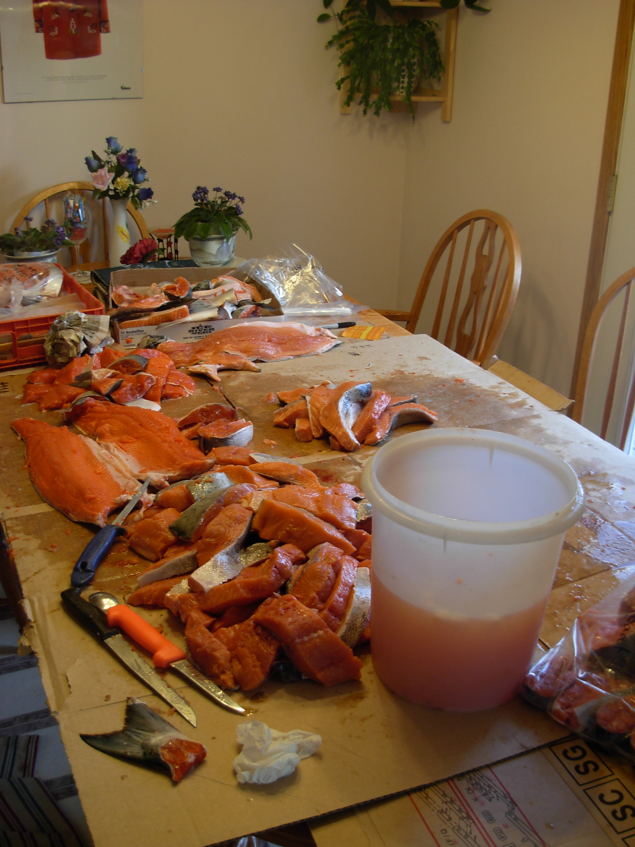
\includegraphics[width=0.7\textwidth]{figures/schreyer-fig2}
    \caption{Food Fish (July 2007) is being prepared for the T’aak̲ú K̲wáan Dancers fund raising barbecue at the Atlin Arts and Music Festival}
    \label{schreyer-fig2}
\end{figure}


The Taku River Tlingit participated with their own dance group for the first time in 2006. I volunteered at the dance group’s barbecue at the Atlin Arts and Music Festival in 2006, 2007, and 2009, and they have consistently been very successful. I have also been privileged to join the T'aak̲ú K̲wáan Dancers in Juneau, Alaska for Celebration in 2006, 2008 and most recently, in 2014. During their stay in Juneau, the dance group has also begun to host a salmon barbecue on Sandy Beach on Douglas Island. Historically, this was an important locale for this K̲wáan (Thornton 2012) and they are renewing this coastal connection. Community members have also been renewing their inland Tlingit connection through the hosting of a salmon feast in Teslin, Yukon for the Inland Tlingit Celebration, which has run since 2011 in the odd-numbered years between Sealaska’s Celebrations. At the Inland Celebration, known as Hà Kus Teyea, each of the Inland Tlingit communities (Teslin Tlingit Council, Taku River Tlingit, and Carcross-Tagish First Nation) take turns hosting a feast. The Taku River Tlingit feast features salmon and they also host a salmon filleting contest earlier on the day of the feast, where contestants compete for the fastest filleting and best filleting skill awards.

As can be seen above, salmon helps to promote physical and mental health, as well as social connection. Similarly, in 2007, Wayne Carlick, dance leader and renowned carver, also developed a skit for the children’s dancers, Dikée Aankáawu Yátx’i (Children of the Creator), at the Atlin Arts and Music Festival that illustrated the ceremony associated with the first salmon caught each year down river. In this ceremony, to respect the salmon after it is eaten, the bones are placed back in the water to replenish the salmon for future generations. As Lakoff and Johnson write, “the metaphors we live by, whether cultural or personal, are partially preserved in ritual” (Lakoff and Johnson 1980: 234). Salmon, the bloodline of the Taku people, is therefore also helping to feed the spiritual and cultural well-being of the Taku River Tlingit people, as well as their physical well-being.

The connection between the Taku River and community health can also be seen in the community’s desire to keep the land healthy. In the Lands and Resources Department’s

Vision and Management document, Hà t\_tátgi hà khustìyxh - Our Land is Our Future, it is written, “Just as without land we cannot exist, without healthy land we can not be healthy people” (2003: 17). It is the land, particularly the Taku River, which makes people feel good and stay healthy. Terry Jack, who I mentioned earlier, told me that during the winter he misses the Taku and being on the land, and how he feels restless until he’s there again. Other people have mentioned this to me as well. Andy Williams, a former Spokesperson and Wolf Clan director and one of Mrs. Nyman’s sons, is another person who has told me about the connection he feels to the Taku River. Andy, who lives in Whitehorse, has said that he tries to get to the Taku as often as possible in the summer because it feels like home and his roots are there (Schreyer field notes 2006). During an interview with Sandra Jack, the Spokesperson or leader of the Taku River Tlingit First Nation in 2006, I asked if she ever has the time to make it to the Taku. Sandra replied:

\begin{quote}
I haven’t [been lately], no, but I’ve been down to the Taku. I did a fishing season when I was down there. It was really good because I ended up commercial fishing, and it was just a beautiful time. A lot of people talk about how it changes your life...or it really helps you to heal up more so you can get through the rest of the year, and do reasonably well, and take care of the other part of your life. For myself, I ended up going down there knowing that it was a special place, but not knowing really what to expect. I’d never commercial fished, you know, I’d never been out on the river.... I think what was really important though, what I walked away with was just that experience of being down the Taku, and there were a lot of people that were down there at the time, I think there might have been twenty Tlingits that were all commercial fishing. So, it was something new that we were all trying, not that we knew exactly what we were doing, we just knew that we’d done it before. I mean it’s got to be in our blood (laughing). So, we ended up getting down there and just getting out and enjoying the land, and enjoying the work. [Jack interview September 2006]
\end{quote}

From the above examples, it should be evident that the metaphor of the Heart of the Taku has been expanded amongst community members from knowledge of the landscape to the actions of individuals and I now discuss the implications for the community as a whole.

\section{Metaphors as Social Action}

Basso in his work on the hunting metaphors of the Western Apache people has written that, “one of the properties of any successful metaphor is that is can be refined and enlarged in different ways” (Basso 1996: 60). Potter has commented similarly that, “conceptual metaphors are generally imbricated---that is, overlapping and reinforcing---and operate at a variety of scales” (Potter 2003: 325). This can be seen in the expanded and extended metaphors of the Heart of the Taku that are used amongst the members of the Taku River Tlingit First Nation. While some might argue a connection to metaphor might be lost as the name is translated from the Tlingit T'aak̲ú Téix̲'i to the English meanings of the words, I disagree. English has become the language of the community and is the language that is most often used to promote stewardship throughout their territory. Darnell observed the role of English as a language for social action, when she argued that:

\begin{quote}
In the absence of political, economic, and personal empowerment, language comes to the forefront of the new traditionalism as a powerful symbol of Native-ness, of the right to reclaim lost skills and ways of life…But language enters the equation in another way which is at least as interesting. That is, language is also discourse, a discourse of social action and political empowerment. It is a discourse in English. [Darnell: 1994: 75]
\end{quote}

As noted above, the Taku River Tlingit First Nation has been a role model for other Indigenous communities in terms of their many court cases, documents, and government-to-government negotiations that promote themselves as the rightful stewards of their lands. Paul Nadasdy writes about the members of the Kluane Lake First Nation to the north in the Yukon:

\begin{quote}
If, in the context of the modern nation-state, aboriginal people wish to claim some form of control over their lands, and they wish those claims to be seen as legitimate by others, they must as Richard Handler puts it, speak “in a language that power understands” (1991: 71). And that language is, and has long been, the language of property. [Nadasdy 2002: 253]
\end{quote}

The language of property in this area of Canada is English and the Taku River Tlingit First Nation therefore use English geographic names to convey their own cultural concepts of property and heritage. In this way, the members of the Taku River Tlingit First Nation are using English, as well as Tlingit, to their advantage through the use of these metaphors and through performatives of stewardship. My definition of “performatives of stewardship” is \textit{actions that assert leadership and responsibility in caring for a community’s lands and resources and (re)define who has this responsibility in a particular territory. }This definition is based on Sullivan’s (2006) ideas “performatives of sovereignty” and is highly linked to the Taku River Tlingit First Nation’s own definitions of stewardship, which are outlined in their Vision and Management documents (TRTFN 2003). \

Austin examined the performative nature of language in his book How to Do Things with Words (1962). He described the way that “the issuing of an utterance is the performing of an action” (Austin 1962: 6). Austin separated utterances into illocutionary force (what the utterance does) and perlocutionary force (how the audience reacts). However, Mac Cormac writes that metaphors “often seem to fuse these into a single feature of language” (Mac Cormac 1985: 160). Mac Cormac sees metaphors then as a type of speech act, where one metaphorizes. He writes that:

\begin{quote}
Metaphors not only convey and stimulate meanings, but also perform significant actions. Metaphors suggest, convey, and generate emotions; puzzle; and often form an intimate bond between speaker and hearer (Mac Cormac 1985: 179).
\end{quote}

When this meaning moves beyond the individual to the larger community Mac Cormac says, “we can discover an additional dimension of meaning – that of cultural meaning” (Mac Cormac 1985: 178). This cultural meaning can be seen in the ways that the Taku River Tlingit community members have taken on the historical metaphor of the Heart of the Taku and applied it to contemporary physical, social, cultural, and economic domains. As I have written elsewhere, the genres of place that Taku River Tlingit community members use to promote stewardship in their territory can be seen as performatives of stewardship (Schreyer 2016). The polysemic, imbricated metaphors that are tied together via two languages are another performative of stewardship that community members are involved in, but these are tied to a very specific locale---the island, T'aak̲ú Téix̲'i or the Heart of the Taku.

\section{Conclusions}

Thornton, in the abstract for his chapter entitled, “Language and landscape among the Tlingit”, writes, “although the language is considered endangered, Tlingit toponyms and geographical nomenclature are well documented and many groups continue to occupy and use their traditional territory in ways that support traditional concepts of the lands and waters of their living space” (2011: 275). This is what I have been attempting to show for the specific place, T'aak̲ú Téix̲'i, the Heart of the Taku, located in Taku River Tlingit territory. However, the impact of language endangerment has made this discourse one that is also tied to English. In this chapter, Thornton also argues for a new understanding of the concept of “ecotope” or “the smallest ecologically-distinct landscape features” (Hunn \& Meilleuur 2010: 15ff), in order that, “cultural landscapes may come to be understood not simply as named sites but as a composition of meaningful places within a sociological system” (276). Thornton discusses islands as one particularly relevant type of ecotope within Tlingit society (2011: 284). Therefore, throughout this in-depth discussion of the numerous ways that the Heart of the Taku is understood and used by Taku River Tlingit community members, I feel that we can use this specific island as a case study of Thornton’s concept. Thornton includes four processes that affect how ecotopes are viewed and understood. These are: perception, affordance, practice, and biospiritual forces (2011). I, therefore, review each of these processes in reference to the discussion provided above about the Heart of the Taku in order to discuss the specific ecotope of the Heart of the Taku.

First, Thornton discusses perception or the different ways that aspects of the landscape are categorized. Using the concept of embodiment from phenomenology, Thornton writes that:

Given this logic and the primacy of the body as instrument of landscape perception, we would expect to find widespread metaphorization and anatomical referencing of the body in the landscape. Indeed this is the case in Tlingit… (Thornton 2011: 278).

Thornton goes on to discuss the types of body parts that are referenced in Tlingit, which generally are those focusing on the head, and are often orifices. In his other work, Thornton has commented in regards to anatomical metaphors that Tlingit speakers seem to have a “marked preference for naming places after external bodily features, as opposed to internal ones” (2008: 97). He does note, however, the heart is one of the few internal organs he has seen represented (2008: 215). In terms of perception, the Heart of the Taku, is classified in relation to body parts, like many other Tlingit names, although it seems that its reference to an internal organ is rather special. Similarly, we should remember that the internal organ in question belongs to a giant, who is a powerful being from a different time period, rather than a human or an animal, and this may invoke different forms of perception.

Next, Thornton discusses the concept of affordance, which he describes as “a means of understanding how particular objects or environments ‘invite’ certain action possibilities and constrain others” (2011: 279). In particular, Thornton references Cruikshank’s work (2005), which examines the dialogues that occur between people and glaciers amongst Tlingit and Athapaskan groups (2011: 280). Similarly, a recent Taku River Tlingit community newsletter remarked, “Elders say, the land is alive. We just have to have the conversation. How? Be on the land. Be alive in it. Listen, and Talk” (TRTFN 2009: 1). As well, one of the motivations for the Learning to Talk to the Land participatory mapping project was so that community members could learn how to further develop their stewardship practices through learning how to call the land by its correct name (Schreyer et al 2014). When asked if she thought it was important for people to learn the correct Tlingit place names, Susan Carlick replied, “I think that our land would appreciate it” (Carlick, S., interview, 2011), which again shows that the land is inviting certain actions. T'aak̲ú Téix̲'i was one of the first places to be included within the Taku River Tlingit place names mapping project. There are more pictures included on the website for the Taku River, T'aak̲ú Héen, and T'aak̲ú Téix̲'i than any other place and during the design of the website it was important to our community research partners that photographs of T'aak̲ú Téix̲'i appear in the set of photos that circulate through the website’s cover page. This priority inclusion of T'aak̲ú Téix̲'i continues to illustrate the importance of this particular place name, locale, and ecotope.

The third process that Thornton discusses is practice, which he describes as the way in which people put the possibilities of dialogue from affordance into practice. He also states that, “an ecotope’s utility is a reflection of its practical significance to those who make a living from it” (2011: 281). In this case, the possibility that is enacted through the use of the place name of the Heart of the Taku and all of the associated metaphors is the practice of stewardship and respecting the land and the relationship people have to the land, which includes the plants and the animals that make their homes there. Thornton also states that, “another critical dimension of ecotope conceptualization was cultural keystone species (Garibaldi \& Turner 2004)” (2011: 282). As mentioned above, one of the metaphors that is associated with the Heart of the Taku is the set of extended metaphors of bloodline, lifeblood and lifeline and one of the meanings associated with these is a keystone species from the Taku River, salmon.

Last, Thornton discusses the concept of biospiritual forces, or the animate and powerful spirits that are a part of the landscape. He writes that similar to other animistic societies, “So it is in Tlingit country, where the oceans, rivers, mountains, glaciers, and a variety of other landforms were considered alive or animated by spirits to whom one could appeal (Swanton 1908; de Laguna 1972)” (Thornton 2011: 283). As mentioned previously, the origins of the name the Heart of the Taku come from the mythohistoric time of the giants, but beyond this there is the conception that the land is listening. As well, the respect for the land and the biospiritual forces can be seen in the ceremony, which is performed at the Taku River, where the first salmon bones of the fishing season are put back into the river to help sustain its power and life force.

In sum, T'aak̲ú Téix̲'i, the Heart of the Taku, fits well within Thornton’s concept of an ecoptope. The metaphors that the community members are using are further embedding their concepts of stewardship within both the Tlingit language and the language of English through the processes of perception, affordance, practice, and biospiritual forces. In his discussion of performatives, Austin (1962) also discussed what he called “the felicity condition”, which means that in order for the performative to be completed it has to be both heard and understood to be a performative by the listener. As the language of stewardship in this community has often been tied to English, performatives through English metaphors are a necessary part of this felicity condition. As a result, the multi-layered meanings of T'aak̲ú Téix̲'i, and specifically, the English Heart of the Taku, means that insiders and outsiders to the community may have a different understanding of this ecotope depending not only on where they stand, but where their ancestors have stood and how they have engaged this landscape since time immemorial.




\section*{Acknowledgments}

I would like to say gunalchéesh, thank you, to the members of the Taku River Tlingit First Nation for being my research partners and friends. I am honored to work with you and learn from you. I would also like to thank Gary Holton and Thomas Thornton for asking me to participate in this volume honoring James Kari. I am grateful to the two reviewers who provided feedback on my paper; any remaining errors are mine alone. Financial support for this research was provided by: SSHRC, the Northern Scientific Training Program, the Canadian Circumpolar Institute, and the University of British Columbia.


\refheading
\begin{hang}


Austin, J.L. 1962. \textit{How To Do Things With Words}. Oxford: Clarendon Press.

Basso, Keith. 1996. \textit{Wisdom Sits in Places: Landscape and Language Among the Western Apache.} Albuquerque: University of New Mexico Press.

BC Parks. 2012. Taku River/T’akú Téix’ Conservancy  \url{http://www.env.gov.bc.ca/bcparks/explore/cnsrvncy/taku-rv/}, accessed September 5, 2014.

Canadian Press. 2015. BC Upholds Environmental Certificates for Controversial Mines. January 14, 2015  \url{http://www.ctvnews.ca/business/b-c-upholds-environmental-certificates-for-controversial-mines-1.2189673}

Crippen, Julie. 2010. The New Tlingit Dictionary: An Encyclopedia Dictionary of the Tlingit Language. Unpublished document: \url{http://www.drangle.com/~james/dictionary/}

Cruikshank, Julie.  2005. \textit{Do Glaciers Listen? Local Knowledge, Colonial Encounters and Social Imagination}. Vancouver: UBC Press.

Darnell, Regna. 1994. Private Discourse, Public Discourse, and Algonquian Oral Tradition. In Papers of the Algonquian Conference -Volume 25. W. Cowan, ed. Pp. 72-82. Ottawa: National Museum of Canada.

de Laguna, Frederica. 1972. \textit{Under Mount St. Elias: The History and Culture of the Yakutat Tlingit}. 3 vols.  Washington DC: Smithsonian Institute Press.

EcoJustice. 2014. BC Government Violated duty to consult Taku River Tlingit Regarding Controversial  Tulsequah Chief Project. \url{http://www.ecojustice.ca/media-centre/press-releases/bc- government-violated-duty-to-consult-taku-river-tlingit-regarding-controversial-ulsequah-chief-project}

Garibaldi, Ann \& Nancy Turner. 2004. Cultural Keystone Species: Implications for Ecological Conservation and Restoration.  \textit{Ecology and Society} 9(3). 1-18.

Goldschmidt, Walter, Theodore, Haas \& Thomas Thornton. 1998.  \textit{Haa Aaní – Our Land: Tlingit and Haida Land Rights and Use}. Seattle: University of Washington Press.

Handler, Richard. 1991. Who owns the Past? History, Cultural Property, and the Logic of Possessive  Individualism. In Brian Wallace (ed.), \textit{The Politics of Culture},  63-74. Washington DC: Smithsonian Institute Press.

Hunn, Eugene S. \& B. Meilleur. 2010. Toward a Theory of Landscape Ethnoecological Classification. In Leslie M. Johnson \& Eugene S. Hunn (eds.), \textit{Landscape Ethnoecology},  15-26. New York: Berghan.

Indian Country Today Media Network. 2011. Taku River Tlingit First Nation Balances Stewardship with Development in Historic Deal with B.C. \url{http://indiancountrytodaymedianetwork.com/2011/08/13/taku-river-tlingit-first-nation-balances-stewardship-development-historic-deal-bc-46972}, accessed January 17, 2014

Kari, James. 1996a. A Preliminary View of Hydronymic Districts in Northern Athabaskan Prehistory. \textit{Names} 44(4). 253-271.

Kari, James. 1996b.  Names as Signs: ‘Mountain’ and ‘Stream’ in Alaskan Athabaskan Languages. In E.  Jelinek, S. Midgette, K. Rice \& L. Saxon (eds.), \textit{Athabaskan Language Studies, Essays in Honor of Robert W. Young}, 443-75. Albuquerque:  University of New Mexico Press.

Lakoff, G \& Mark Johnson. 1980. \textit{Metaphors We Live By}. Chicago: University of Chicago Press.

Mac Cormac, Earl R. 1985. \textit{A Cognitive Theory of Metaphor}. Cambridge: The MIT Press.

Nadasdy, Paul. 2002. “Property” and Aboriginal Land Claims in the Canadian Sub Arctic: Some  Theoretical Considerations. \textit{American Anthropologist} 104(1). 247-261.

Nyman, Elizabeth \& Jeff, Leer. 1993. \textit{Gágiwduł.àt: Brought Forth to Reconfirm: The Legacy of a Taku River Tlingit Clan}.
 Whitehorse \& Fairbanks: Yukon Native Language Centre \& Alaska Native Language Center.

Potter, James M. 2003. Creation of Person, the Creation of Place: Hunting Landscapes in the American Southwest. \textit{American Antiquity} 69(2). 322-338.

Rivers Without Borders. 2014. Lawsuit from Taku River Tlingit First Nation Threatens Proposed Tulsequah Chief  Mine. \url{http://riverswithoutborders.org/blog/2014/02/lawsuit-from-taku-river-tlingit-first-nation-threatens-proposed-tulsequah-chief-mine}, accessed September 5\textsuperscript{th}, 2014

Schreyer, Christine. 2016. Taku River Tlingit Genres of Places as Performatives of Stewardship. \textit{Journal of Linguistic Anthropology} 26(1). 4--25.

Schreyer, Christine. 2014. Canadian Geography as National Identity: Hudson’s Bay Company Place Names and  their Aboriginal Counterparts. \textit{International Journal of Canadian Studies} 49(1). 315--34.

Schreyer, Christine, Jon, Corbett, Nicole, Gordon \& Colleen Larson. 2014. Learning to Talk to the Land: Online Stewardship in Taku River Tlingit Territory. \textit{Decolonization: Indigeneity, Education, and Society } 3(3). 106--133.

Swanton, John R. 1908. Social condition, beliefs, and linguistic relationships of Tlingit Indians. In \textit{Twenty-sixth Annual Report, Bureau of American Ethnology}, 391-485. Washington DC:  Government Printing Office.

Sullivan, Kathleen M. 2006. (Re)Landscaping Sovereignty in British Columbia, Canada. \textit{PoLAR: Political and Legal Anthropology Review}  29(1). 44-65.

Supreme Court of Canada. 2004. Taku River Tlingit First Nation v. British Columbia (Project Assessment Director), [2004] 3 S.C.R. 550, 2004 SCC 74

Taku River Tlingit First Nation and BC Wild. 1997. Taku: Will a short-lived mining project sever the \textit{bloodline }of the Tlingit people? Booklet.

Taku River Tlingit First Nation. 2014. Aboriginal Languages Initiative Assessment. \url{http://maps.fphlcc.ca/node/3152}

Taku River Tlingit First Nation. 2011. Wóoshtin wudidaa - Atlin Taku Land Use Plan. Atlin, British Columbia.

Taku River Tlingit First Nation. 2009. Tlatsini Map. Atlin, British Columbia.

Taku River Tlingit First Nation. 2007. Mining Policy. Atlin, British Columbia.

Taku River Tlingit First Nation. 2003. \textit{Our Land is Our Future - Hà t\_tátgi hà khustìyxh. Vision and Management Document for the Taku River Tlingit First Nation Lands and Resources Department.} Atlin, British Columbia.

Taku River Tlingit First Nation. 1997. Taku. Film.

Taku River Tlingit First Nation. 1993. Constitution. Atlin, British Columbia.

Taku Wild. 2014. \url{http://www.takuwild.com/}

Thornton, Thomas F. 2008. \textit{Being and Place Among the Tlingit}. Seattle, WA: University of Washington Press.

Thornton, Thomas F.. 2011. Language and Landscape among the Tlingit. In David. M. Mark, Andrew, G Turk, Niclas Burenhult \& David Stea (eds.), \textit{Landscape in Language: Transdisciplinary Perspectives},  289-304. Amsterdam/Philadelphia: John Benjamins.


Thornton, Thomas F.  2012. \textit{Haa Leelk’w Has Aaní Saax’u: Our Grandparents’ Names on the Land}. Juneau \&  Seattle: Sealaska Heritage Institute and University of Washington Press.

Williams, Jackie. 2013. \textit{Lingít Kusteeyí: What My grandfather taught me}. Atlin, BC: Taku River Tlingit First  Nation.


\end{hang}

\begin{center}
\textbf{List of Interviews}
\end{center}

\begin{hang}
Carlick, Alice. 2006. Interview with Christine Schreyer. Atlin, British Columbia, June, 2006.

Carlick, Susan. 2011. Interview with Christine Schreyer. Atlin, British Columbia, June 2011

Gordon, Louise. 2006. Interview with Christine Schreyer. Atlin, British Columbia. June, 2006.

Jack, Sandra. 2006. Interview with Christine Schreyer. Atlin, BC, September 2006

\end{hang}

\bigskip

\orcidfooter{Christine Schreyer}{christine.schreyer@ubc.ca}{}

\label{schreyer-ch-end}
